\section{Experimental Results}
In this section we present the experimental results for supporting the effectiveness of inspection strategy for improving the solution quality of local DFO methods. We also provide the comparison between the local method equipped with inspection strategy and a global method, to emphasize the advantage of ease of exploitation of the structure of the problem, \emph{i.e.}, the room for the choice of more suitable local DFO methods on the user's end.

\subsection{Spurious Local Minima}
The first example 
Quadratic Plus Sine function 
\begin{equation*}
    f(x) =  \sum_{i=1}^{d} \left(x_i^2 + 0.2 \sin(10\pi(x_i - \frac{1}{20}) + 0.2 \right)
\end{equation*}
\begin{figure*}
    \centering
    \raisebox{-0.5\height}{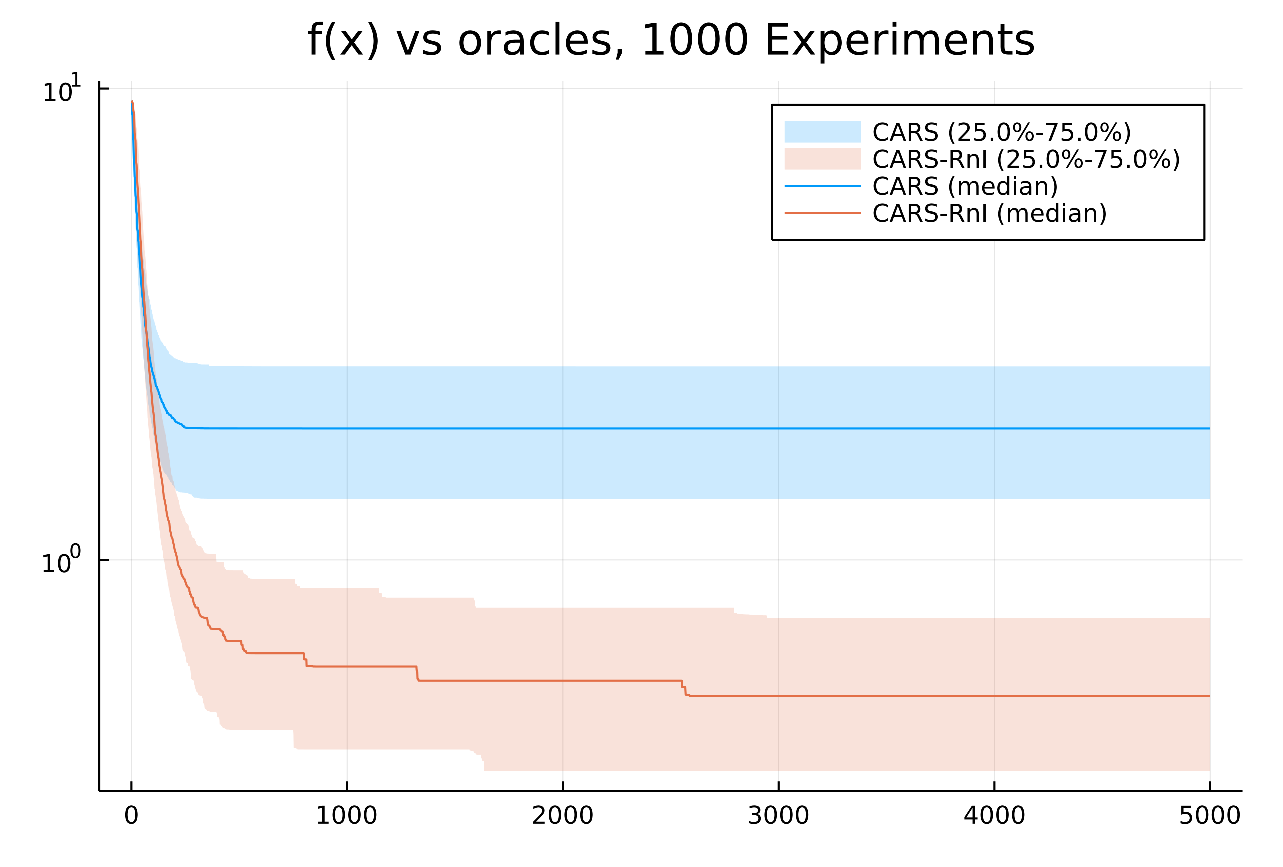
\includegraphics[width=0.48\linewidth]{freq10_amp0.2_quad_plus_sin.eps}}
    \raisebox{-0.5\height}{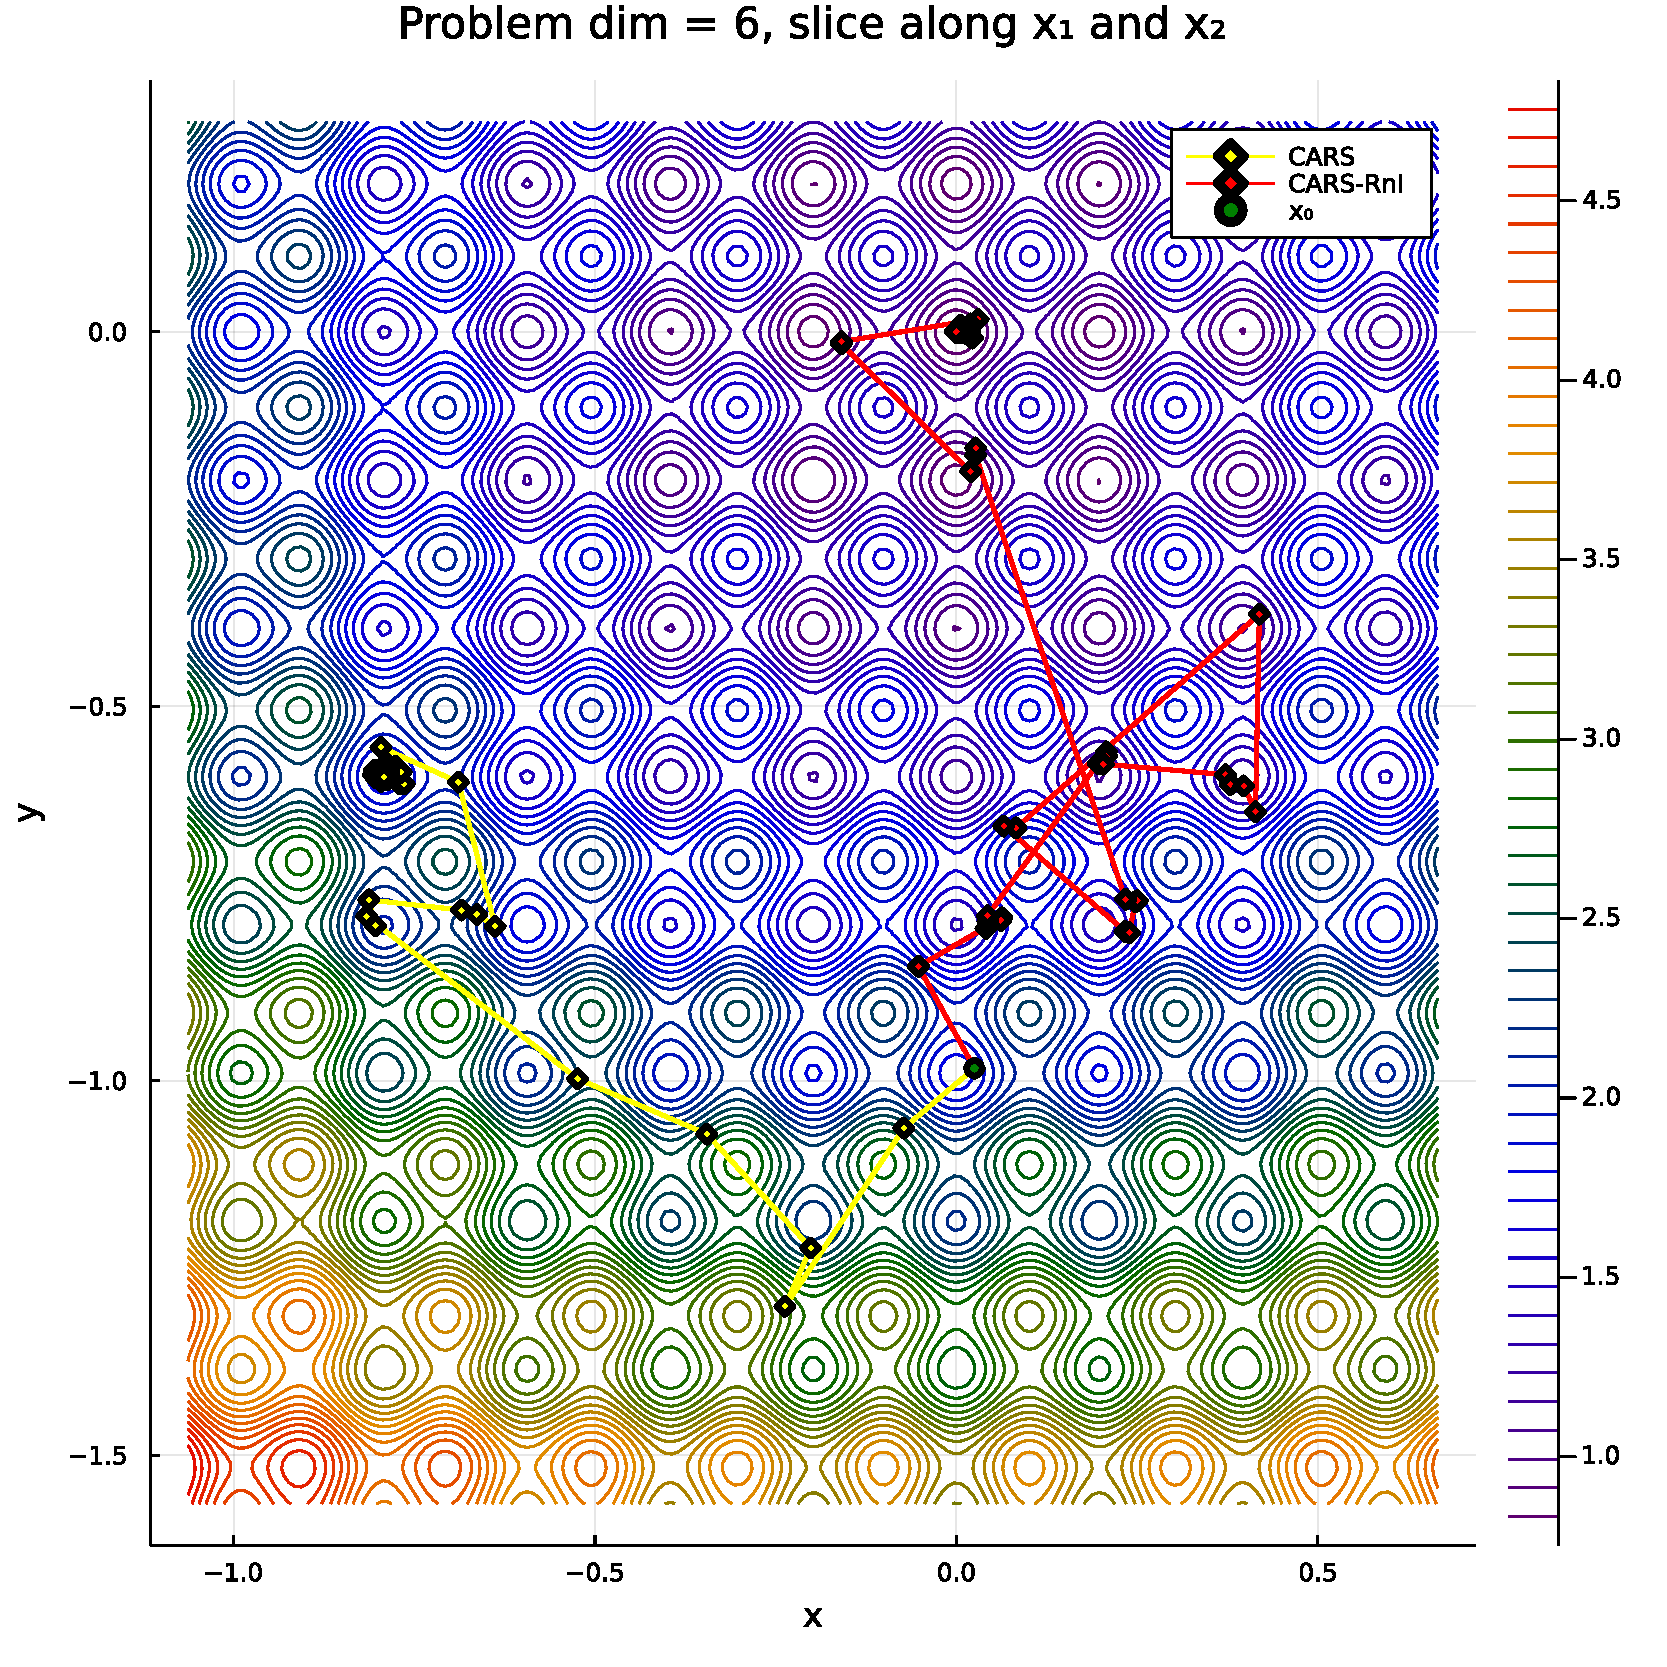
\includegraphics[width=0.48\linewidth]{freq10_amp0.2_quad_plus_sin_sols.eps}}
    \caption{Comparison of CARS and the Inspect-as-Running version of CARS for the quad+sine function}
    \label{fig:Convex plus sine}
\end{figure*}

\subsection{Ackley's Functions}
Example from \cite{chen2019run}
\begin{figure*}
    \centering
    \raisebox{-0.5\height}{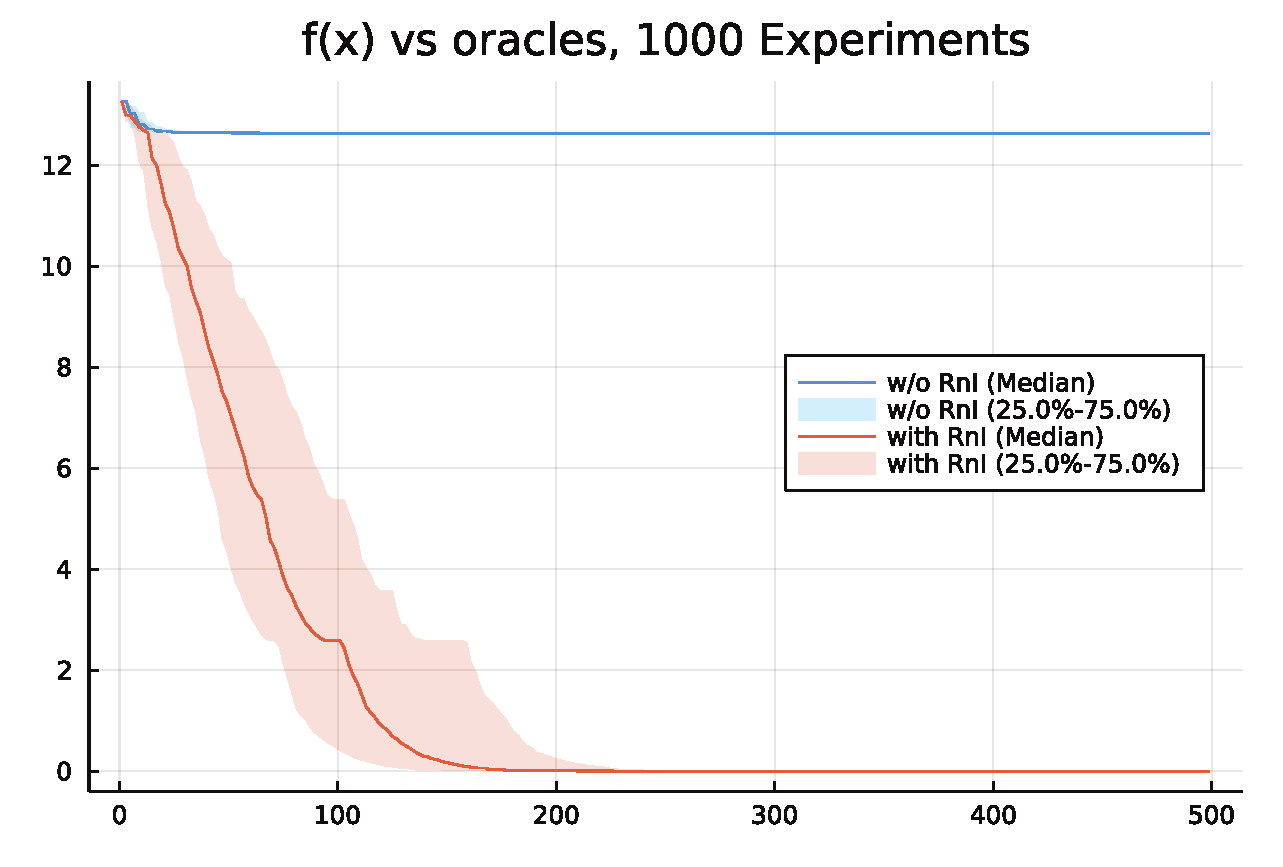
\includegraphics[width=0.48\linewidth]{Ackley.eps}}
    \raisebox{-0.5\height}{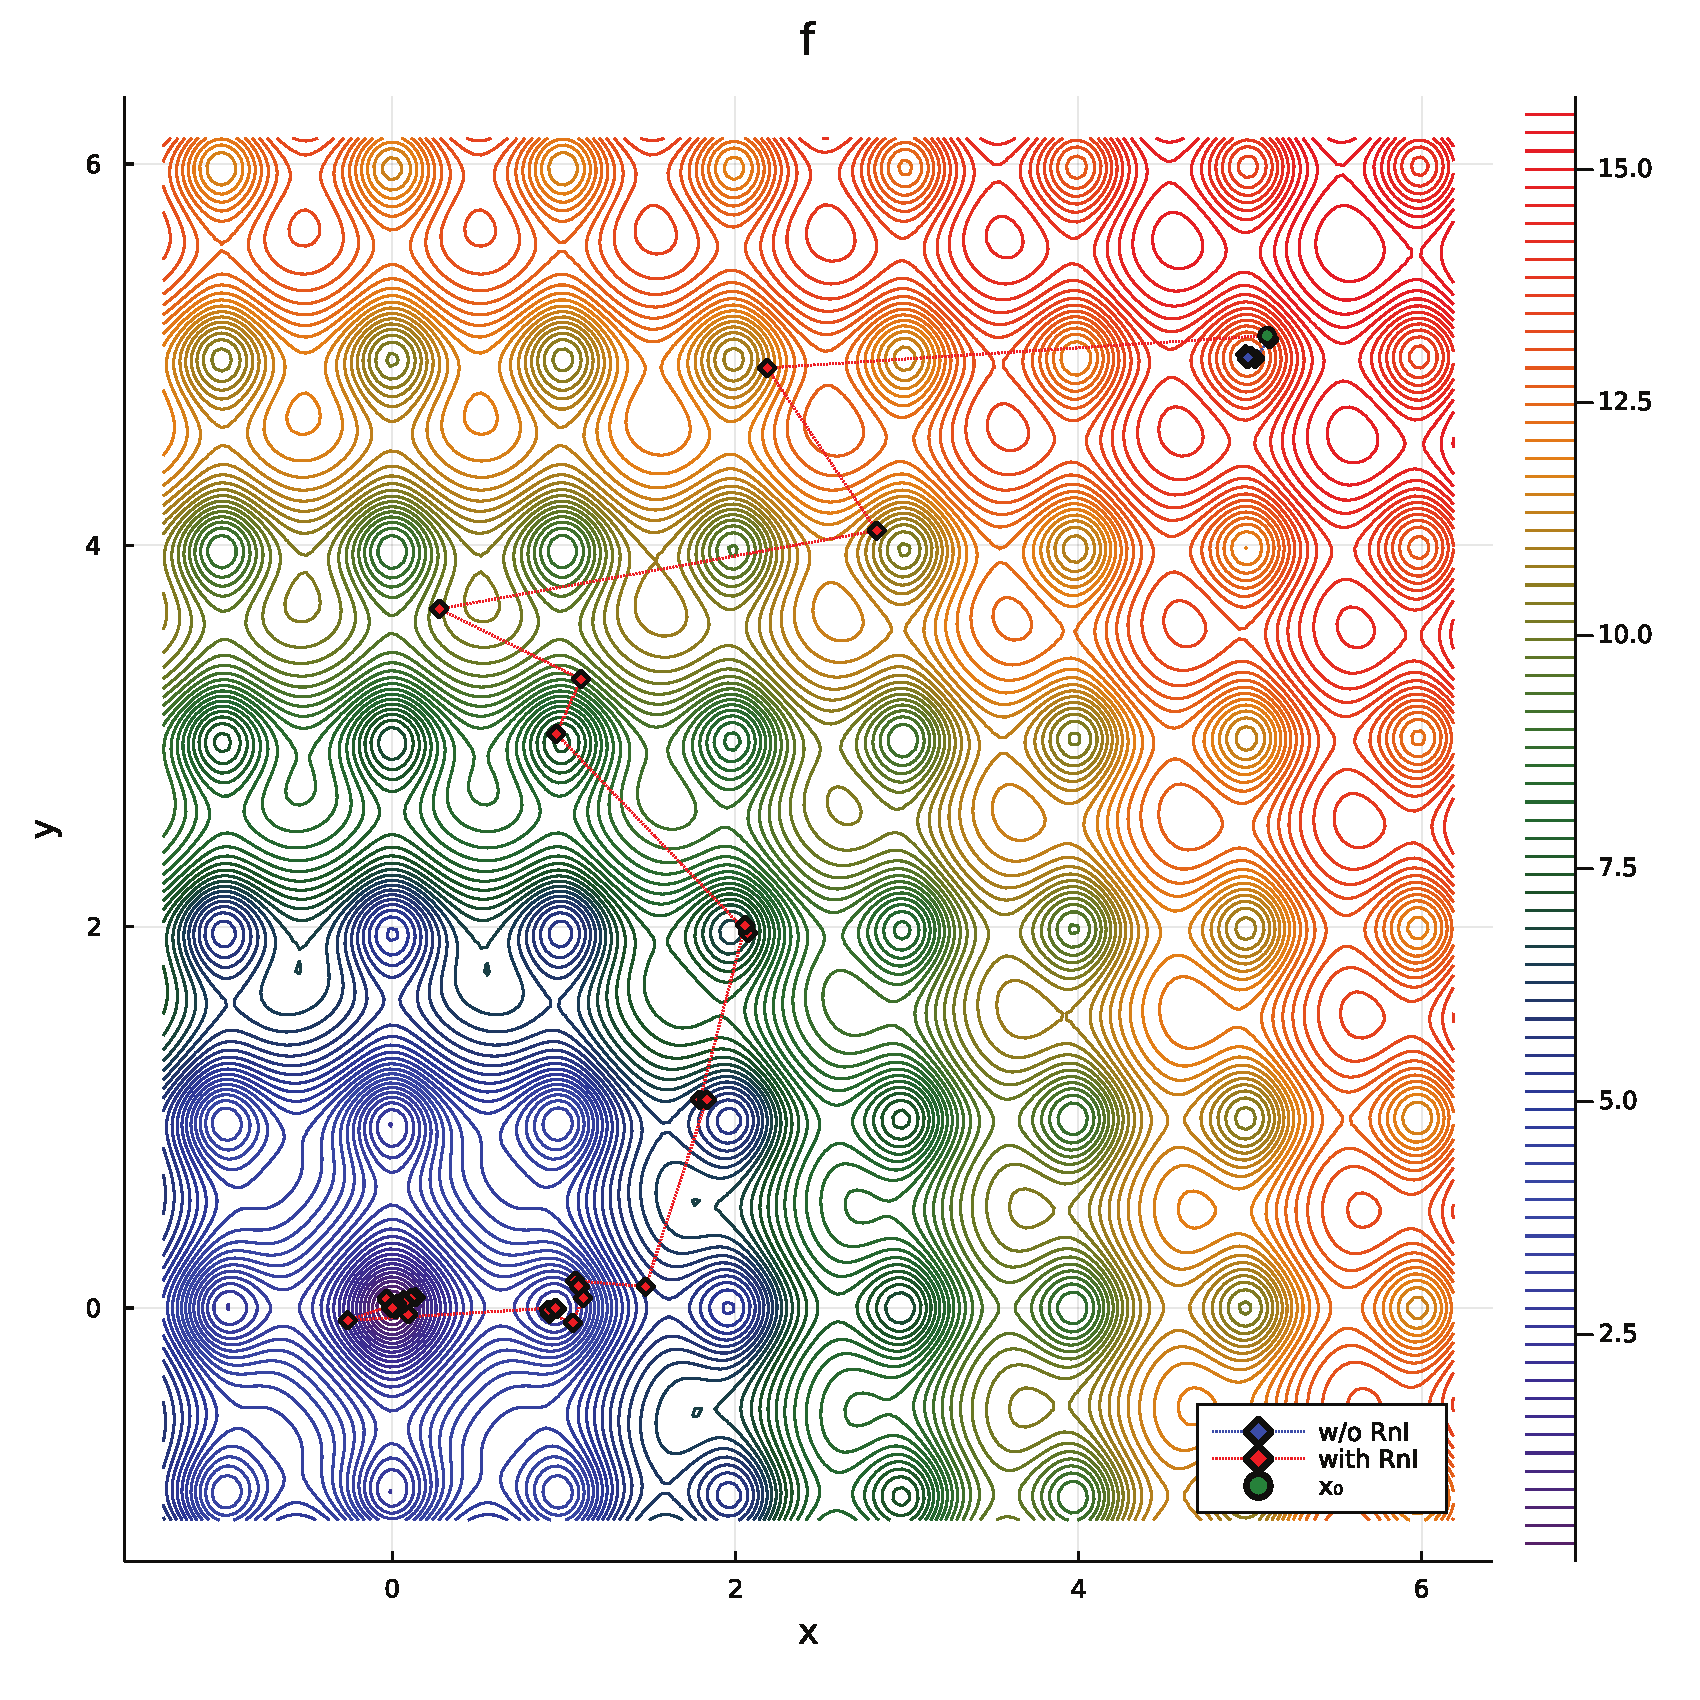
\includegraphics[width=0.48\linewidth]{Ackley_sols.eps}}
    \caption{Comparison of CARS and the Inspect-as-Running version of CARS for the Ackley function}
    \label{fig: Ackley}
\end{figure*}

The asymmetric Ackley function from \cite{chen2019run}
\begin{figure*}
    \centering
    \raisebox{-0.5\height}{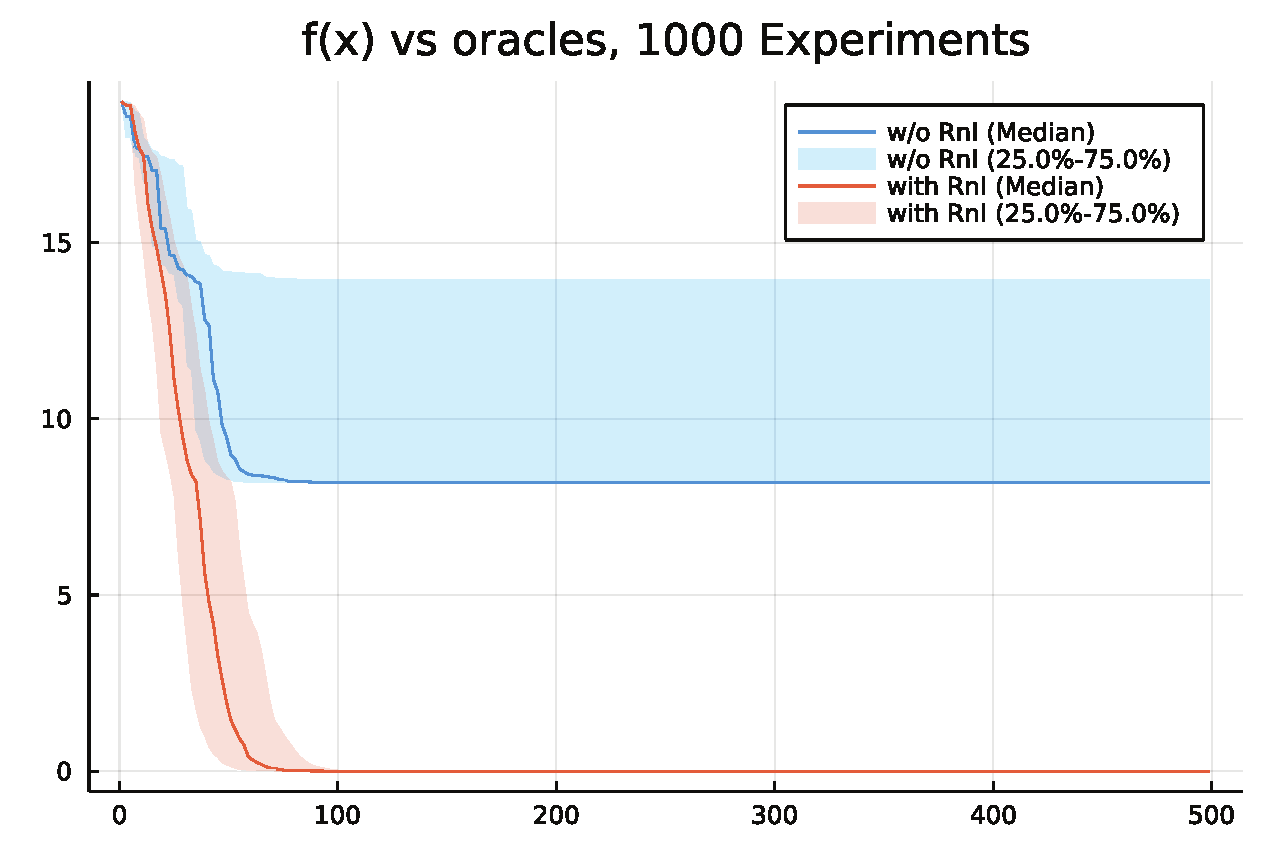
\includegraphics[width=0.48\linewidth]{asym_Ackley.eps}}
    \raisebox{-0.5\height}{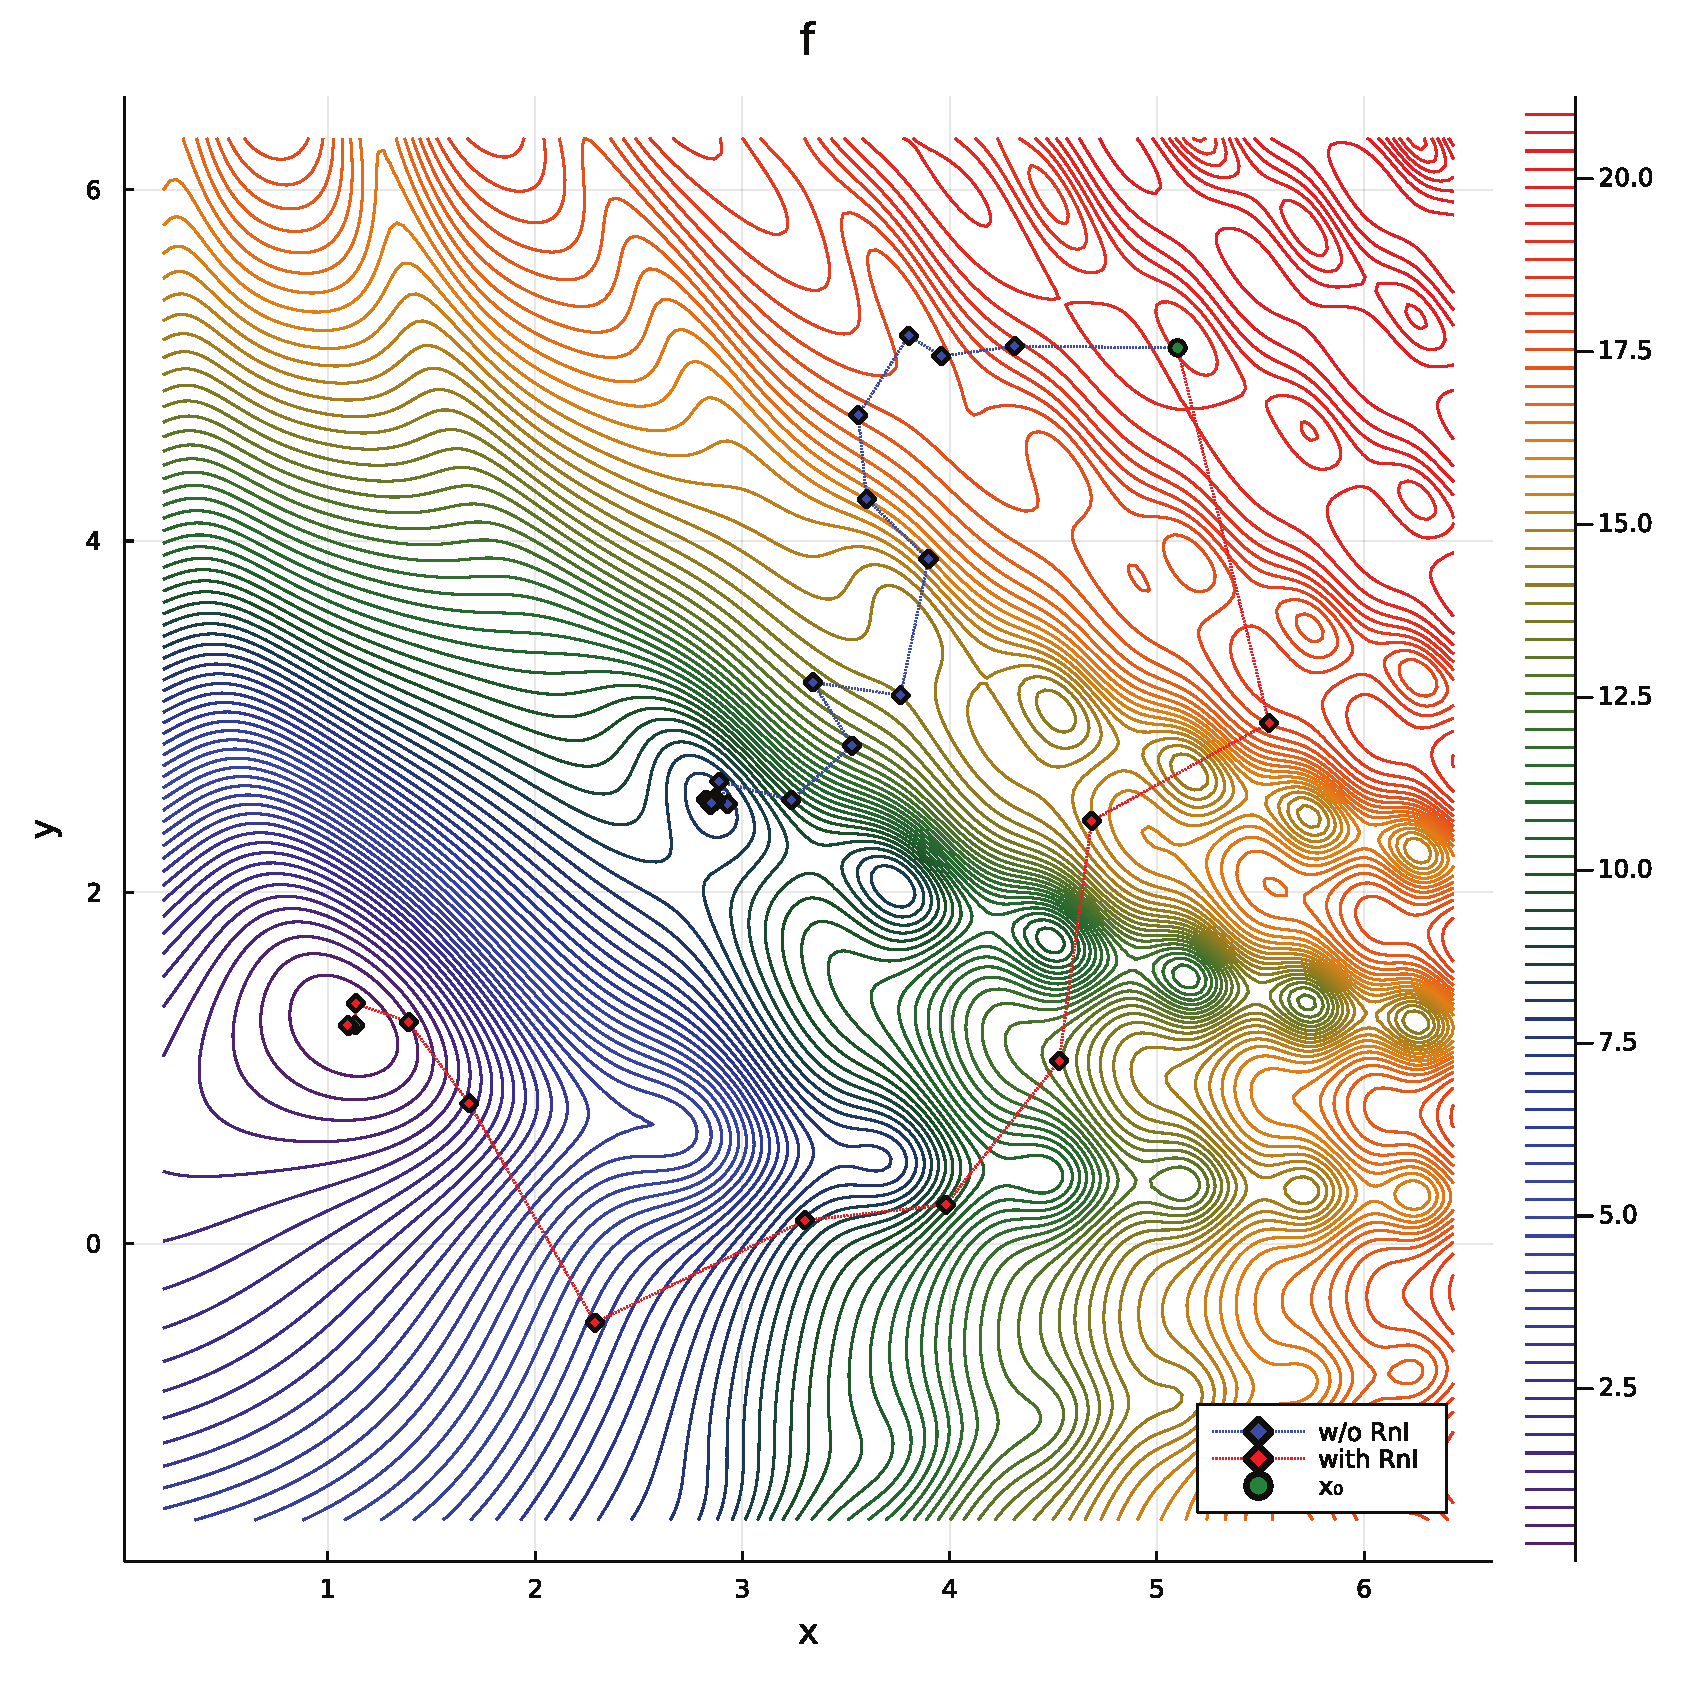
\includegraphics[width=0.48\linewidth]{asym_Ackley_sols.eps}}
    \caption{Comparison of CARS and the Inspect-as-Running version of CARS for the asymmetric Ackley function}
    \label{fig: Ackley asymmetric}
\end{figure*}

\subsection{K-means Clustering}
\subsubsection{Synthetic Gaussian data from \cite{yin2018stochastic}}

\begin{figure*}
    \centering
    \raisebox{-0.5\height}{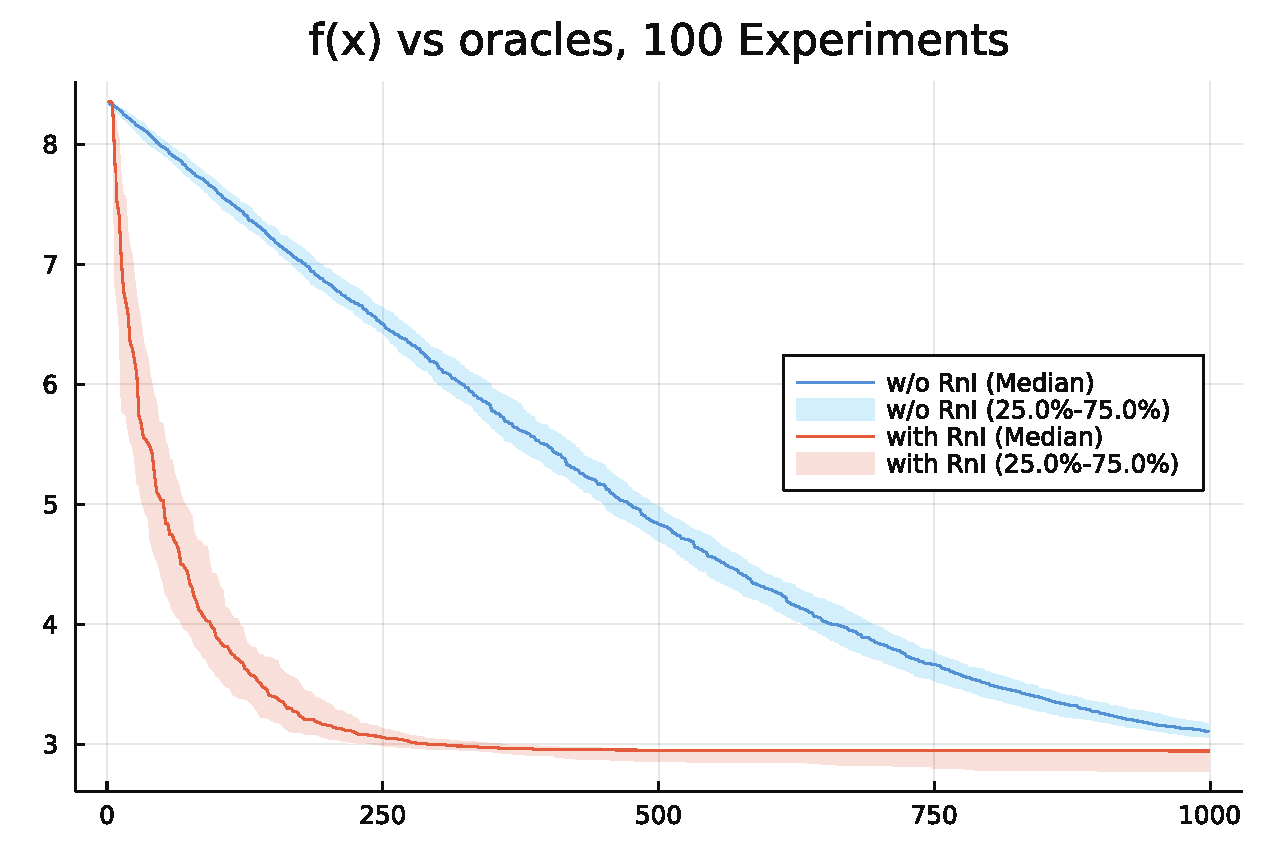
\includegraphics[width=0.48\linewidth]{Kmeans_h0_0.136.eps}}
    \raisebox{-0.5\height}{\includegraphics[width=0.48\linewidth]{Kmeans_h0_0.136_2dplot.eps}}
    \caption{Comparison of CARS and the Inspect-as-Running version of CARS for the K-means clustering problem of synthetic Gaussian data}
    \label{fig: K-means synthetic}
\end{figure*}

\subsubsection{Iris data}
\begin{figure}
    \centering
    \raisebox{-0.5\height}{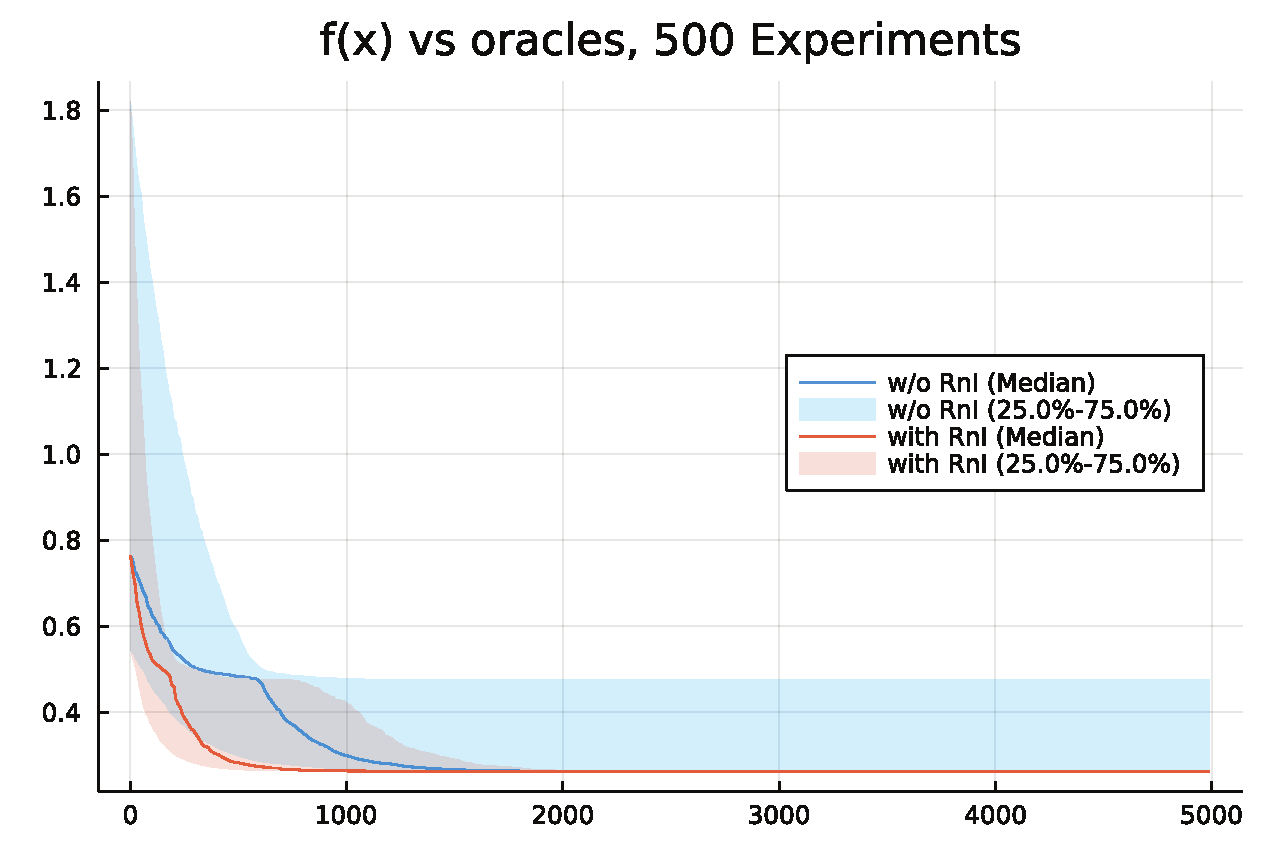
\includegraphics[width=0.48\linewidth]{Iris_h0_1.36e-3_R3.eps}}
    \raisebox{-0.5\height}{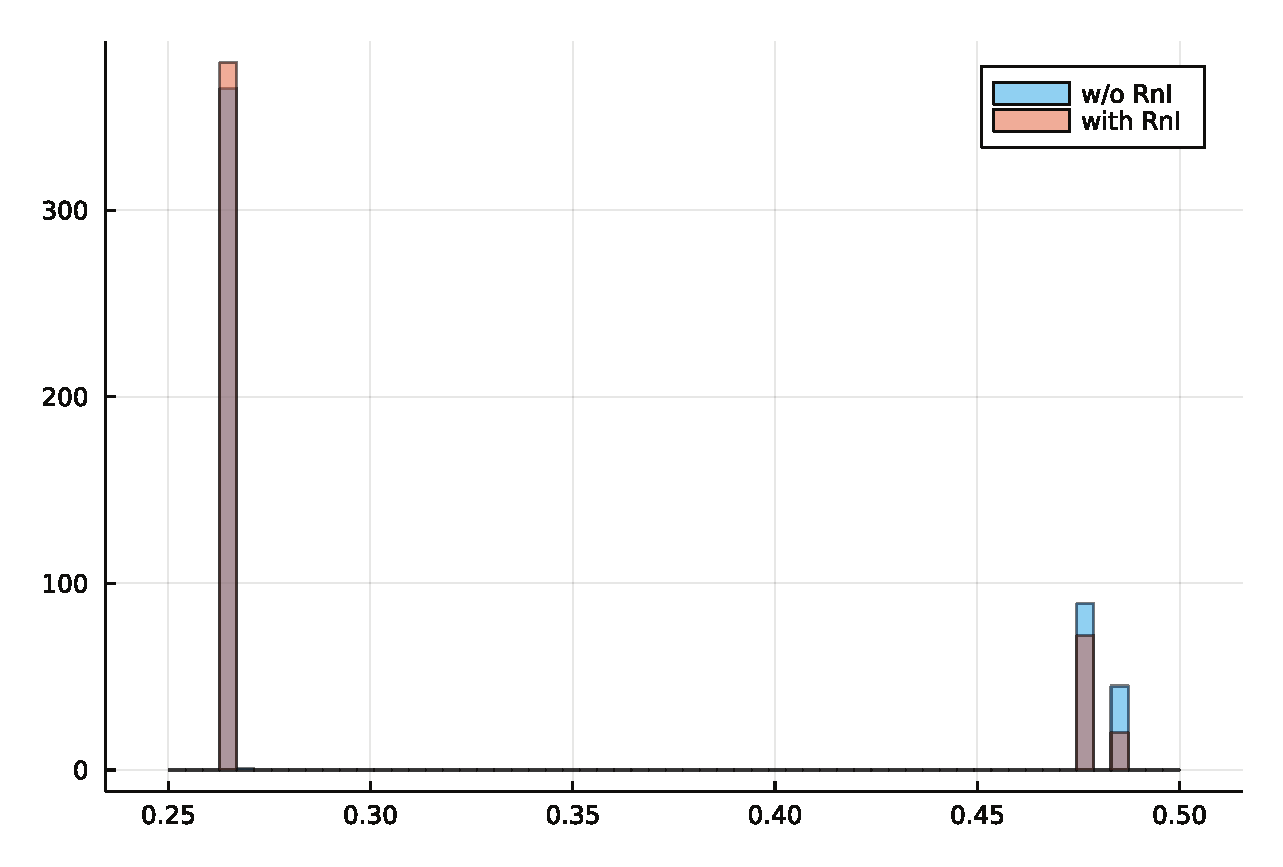
\includegraphics[width=0.48\linewidth]{Iris_histogram.eps}}
    \caption{Comparison of CARS and the Inspect-as-Running version of CARS for the K-means clustering of the Iris dataset}
    \label{fig: K-means Iris}
\end{figure}
\subsection{Nonconvex robust linear regression}

\subsection{Hyperparameter tuning}
Hyperparameter tuning in training a convolutional neural network for classifying the MNIST dataset.
The hyperparameters were $L^2$ regularization parameter in the loss, the learning rate for the optimizer (AdaDelta), and the annealing rate for the scheduler (StepLR). To show the ability to escape the local minima more clearly, we started from a not an excellent point $x_0 = (0.5, 0.5, 0.5)$.

The objective function for the hyperparameter is set to be the mean of two samples, where each measures the misclassification rate of the trained model with the given set of hyperparameters.

\begin{figure}
    \centering
    \raisebox{-0.5\height}{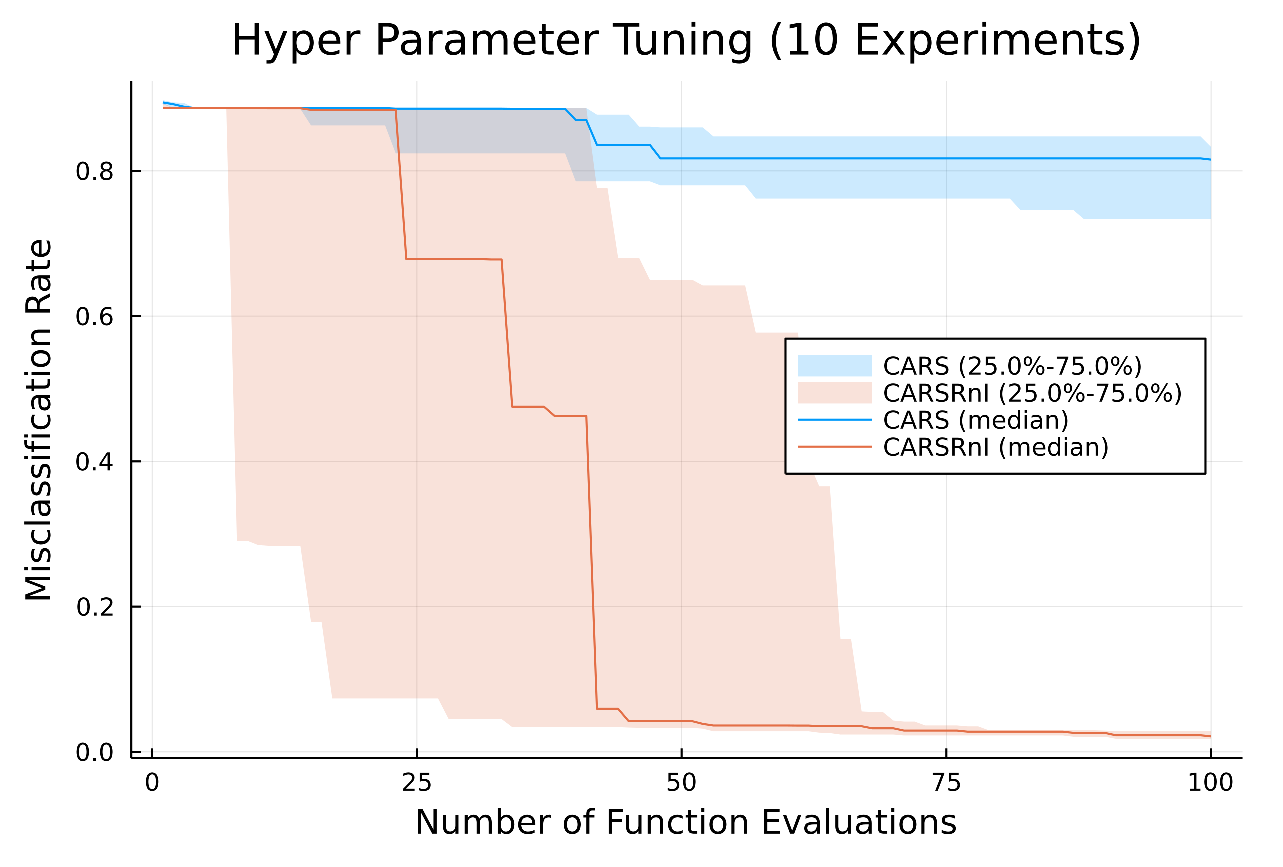
\includegraphics[width=0.48\linewidth]{CARS_vs_CARSRnI_julia.eps}}
    \raisebox{-0.5\height}{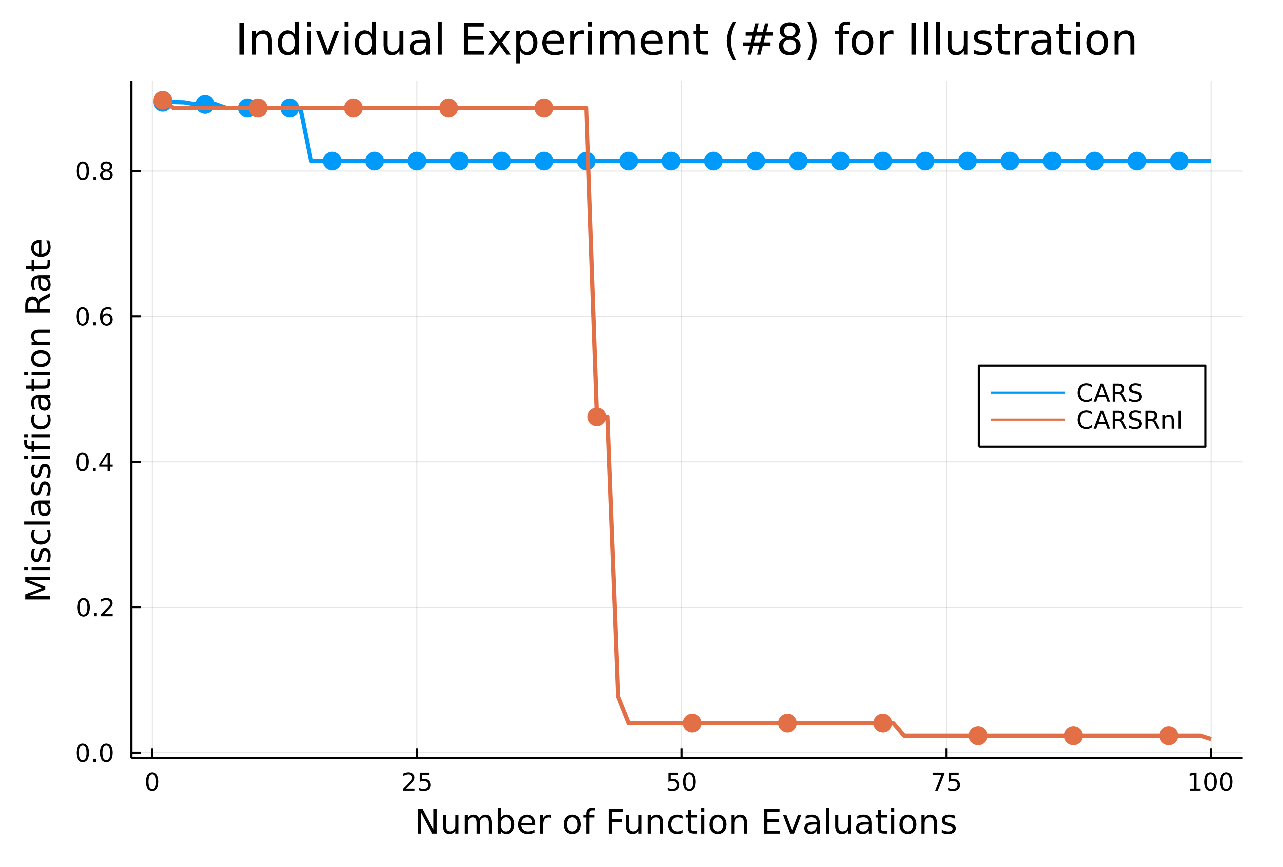
\includegraphics[width=0.48\linewidth]{CARS_vs_CARSRnI_Individual_julia.eps}}
    \caption{Comparison of CARS and the Inspect-as-Running version of CARS for hyperparameter tuning for training a convolutional neural network for MNIST dataset}
    \label{fig: HP Tuning - MNIST}
\end{figure}
